\documentclass{sigchi}
\CopyrightYear{2016}
\setcopyright{acmlicensed}
\doi{http://dx.doi.org/10.475/123_4}
\isbn{123-4567-24-567/08/06}
\conferenceinfo{CHI'16,}{May 07--12, 2016, San Jose, CA, USA}
\acmPrice{\$15.00}
\usepackage{balance}       % to better equalize the last page
\usepackage{graphics}      % for EPS, load graphicx instead 
\usepackage[T1]{fontenc}   % for umlauts and other diaeresis
\usepackage{txfonts}
\usepackage{mathptmx}
% \usepackage{amsmath}
% \usepackage{amsmath,amsfonts,amsthm} 
\usepackage[pdflang={en-US},pdftex]{hyperref}
\usepackage{color}
\usepackage{booktabs}
\usepackage{textcomp}
\usepackage{microtype}        % Improved Tracking and Kerning
\usepackage{ccicons}          % Cite your images correctly!
\usepackage{todonotes}
\def\plaintitle{SIGCHI Conference Proceedings Format}
\def\plainauthor{First Author, Second Author, Third Author,
  Fourth Author, Fifth Author, Sixth Author}
\def\emptyauthor{}
\def\plainkeywords{Authors' choice; of terms; separated; by
  semicolons; include commas, within terms only; required.}
\def\plaingeneralterms{Documentation, Standardization}
\makeatletter
\def\url@leostyle{%
  \@ifundefined{selectfont}{
    \def\UrlFont{\sf}
  }{
    \def\UrlFont{\small\bf\ttfamily}
  }}
\makeatother
\urlstyle{leo}
\def\pprw{8.5in}
\def\pprh{11in}
\special{papersize=\pprw,\pprh}
\setlength{\paperwidth}{\pprw}
\setlength{\paperheight}{\pprh}
\setlength{\pdfpagewidth}{\pprw}
\setlength{\pdfpageheight}{\pprh}
\definecolor{linkColor}{RGB}{6,125,233}
\hypersetup{%
  pdftitle={\plaintitle},
  pdfauthor={\emptyauthor},
  pdfkeywords={\plainkeywords},
  pdfdisplaydoctitle=true,
  bookmarksnumbered,
  pdfstartview={FitH},
  colorlinks,
  citecolor=black,
  filecolor=black,
  linkcolor=black,
  urlcolor=linkColor,
  breaklinks=true,
  hypertexnames=false
}
\begin{document}
\title{\plaintitle}
\numberofauthors{3}
\author{%
  \alignauthor{Leave Authors Anonymous\\
    \affaddr{for Submission}\\
    \affaddr{City, Country}\\
    \email{e-mail address}}\\
  \alignauthor{Leave Authors Anonymous\\
    \affaddr{for Submission}\\
    \affaddr{City, Country}\\
    \email{e-mail address}}\\
  \alignauthor{Leave Authors Anonymous\\
    \affaddr{for Submission}\\
    \affaddr{City, Country}\\
    \email{e-mail address}}\\
}
\maketitle
\begin{abstract}
  TODO.
\end{abstract}
\category{H.5.m.}{Information Interfaces and Presentation
  (e.g. HCI)}{Miscellaneous} \category{See
  \url{http://acm.org/about/class/1998/} for the full list of ACM
  classifiers. This section is required.}{}{}
\keywords{\plainkeywords}

\section{Evaluation}
\subsection{Participants}

As we discussed the experiment design before in section 2.2.1, our user study is conducted in two time slots within a day from 6pm to 8pm as daytime study, and 9pm to 11pm as nighttime study. We recruited 17 participant groups (6 groups of people (M=2.33), 11 individuals (7 male, 4 female)) in total, 10 participant groups (4 groups of people (M=2.25), 6 individuals (4 male, 2 female)) are from day time and 7 participant groups (2 groups of people (M=2.5), 5 individuals (3 male, 2 female)).

All participants are randomly chosen from pedestrians. The group of people are treated as same as individuals since the questionnaires are answered by one person inside the group, or they share consistent answers for their final answer.


\subsection{Quantitative Analysis}

The statistic results of user study questionnaires, as shown in figure 3.1, indicates that 58.8\% of pedestrians showed their reaction to the windshield display; 60.0\% of pedestrians with reactions performs interaction with the display; 50.0\% of pedestrians who showed interaction was in a group; The attention of pedestrians has been drawn by the display in general first stopped and after a short pause walked straight up to the display to
inspect it in detail. The second part of qualitative results gives the pedestrians subjective perspective of the windshield display usability.

For the purpose recognition, 35.3\% of pedestrians understand the purpose, pedestrians received the interpretation correct on their first glance. 82.4\% of pedestrians recognize the display, and 47.0\% of pedestrians recognize the display functionalities, which means the users in total guessed in the right direction of the original intention that either a crosswalk is nearby or the display shall fulfill some kind of security feature to warn about approaching vehicles as well as some users confused the display as an art installation.


\begin{figure}
\centering
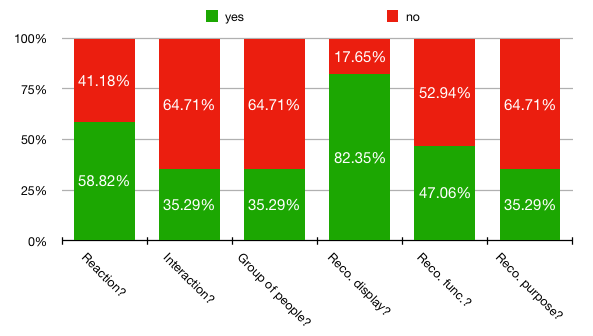
\includegraphics[width=0.9\columnwidth]{figures/yesno}
\caption{\textbf{Pedestrian awareness:} 17 participant groups (6 group people, 11 individuals (7 male, 4 female)), 
58.82\% showed reaction; 60.0\% of reaction people showed interaction with the display; 
82.36\% aware the display; 35.3\% recognize the purpose. }~\label{fig:figure1}
\end{figure}

The figure 3.2 demonstrates the likert scale measurement of the pedestrians subjective perspective on the usability of windshield display, either the warning sign extension or the general purpose of windshield display.  The participants has neutral opinion on this installation security (23.53\%+17.65\% positive versus 23.25\%+17.65\% negative) and doubt the estimation accuracy (17.65\% + 35.29\% negative). For the acceptance of most of the participants (> 70\%) are accepting this installation and willing to install this to their personal cars if it works well (>50%).

To eliminate the effects of daytime study group and nighttime study group, we gives two hypotheses first:  H0: The acceptance of pedestrians from day time group significant bigger than night time; H0: The acceptance of pedestrians from day time group significant smaller than night time. We chose significant level α=0.05 conduct t-test. In the first two H0 hypothesis, p = 0.007 < α; p = 0.021 < α are both less than significant level, we reject both null hypotheses.  With the same procedure, we conduct t-test to the rest of 10 questions (11 questions in total as shown in figure 2) and the statistical significant effects are those for which the zero or null value of the effects lies outside the 95\% confidence interval (i.e., p < 0.05), which proves that there is no significant difference of pedestrians answers from daytime group and nighttime group.

\begin{figure*}
\centering
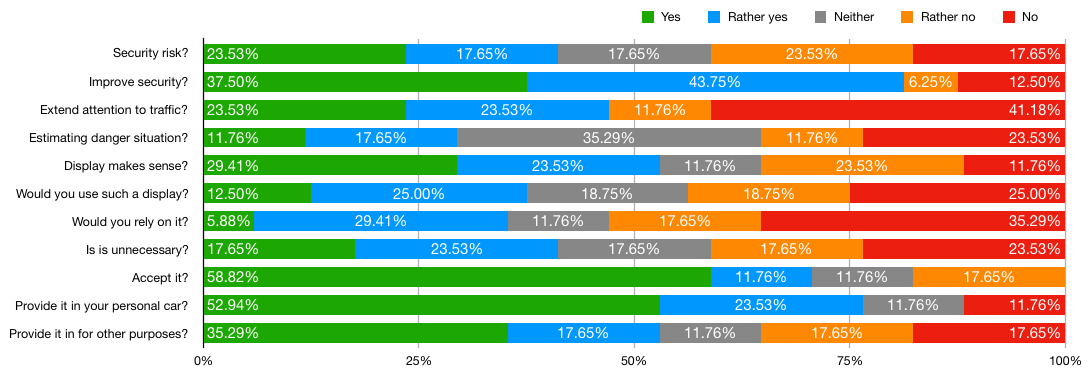
\includegraphics[width=1.75\columnwidth]{figures/likert}
\caption{
    Pedestrians subjective usability: Participants has neutral opinion on this installation (41.18\% vs 41.18\%) 
    and doubt the estimation accuracy (52.94\% negative).
    Pedestrians acceptance: Most of the participants (>70\%) are accepting this installation 
    and willing to install this to their personal cars if it works well.
}~\label{fig:figure2}
\end{figure*}

\subsection{Qualitative Analysis}

In the user study, we also collects the qualitative answers from pedestrians. 

\textbf{Reaction}: Most pedestrians whose attention has been drawn by the display in general first stopped and after a short pause walked straight up to the display to inspect it in detail. In case that no other person was located near the display, the illumination, color coding and blinking effect of the icon in “hazard mode” were mentioned as the most salient features of the installation. The residence of other pedestrians were already located nearby the installation also attracted other pedestrians and created a honeypot effect [CITE: Florian Alt]. 

\textbf{Recognition}: Less than a half of the observed pedestrians got the interpretation right on the first shot. Most users in total guessed in the right direction of the original intention - that either a crosswalk is nearby or the display shall fulfill some kind of security feature to warn about approaching vehicles. Some users were confused about the display and interpreted it as a kind of a street art installation.Most people agreed on the usefulness of the kind of display to improve the overall security for pedestrians in traffic situations. 

\textbf{Security}: Since the technique is new people have to get familiar with it before they rely on it. The technology has to establish and thereby prove to be safe and useful. Most questioned people see the display as a security risk for pedestrians, as long as the technology is too new, not commonly known among public and not completely reliable and tested. Further some people were concerned that, as long as the technology is new, people could be confused and distracted. The illuminated color coding makes people improves awareness of the street situation, especially during night time. The blinking and novel nature of the display made people aware of the street situation. Most participants would use the display if it were an established technology but primarily rely on their own senses. Concerns were mainly expressed regarding possible technical and security issues and users were torn regarding the necessity of the display. 

\textbf{Acceptance}: Some thought the existing traffic lights are sufficient, some agreed on the purpose of improving security next to view-blocking cars. Nevertheless, all participants stated, that they would accept it, in case that an improvement for road safety is proved for the installation and under the condition that the system actually works reliably. Most participants would provide the display in their own car if it is free or offered as a standard feature in cars and to do something good for society. Half the people would not like arbitrary content to be displayed on their personal car windshield.

\textbf{Privacy}: Reasons where disliking of the idea were privacy issues and the indignation of providing personal information in public. In contrary the other half would like the idea of making some money with advertisement. Following other use cases and contents were mentioned to be displayed: traffic news, nearby public transportation connections, objects of interest like cafes or bars, news feeds, advertisement, personal messages to other pedestrians, movies, social media feeds.


\section{Results and Discussion}
\subsection{Outcomes}


\begin{table}
  \small
  \centering
  \begin{tabular}{l l l l l l l}
    % \toprule
    & \multicolumn{3}{c}{\small{\textbf{Day Time}}} & \multicolumn{3}{c}{\small{\textbf{Night Time}}} \\
               \cmidrule(r){2-7}
    REACTION & {\small \textit{Avg.}} & {\small \textit{Med.}} & {\small \textit{SD}} & 
      {\small \textit{Avg.}} & {\small \textit{Med.}} & {\small \textit{SD}} \\
    \midrule
    Interview & 223.0 & 44 & 432,321 & 223.0 & 44 & 432,321 \\
    Observation & 22.2 & 16 & 234,333 & 223.0 & 44 & 432,321\\
    % \bottomrule
  \end{tabular}
  \caption{Table captions should be placed below the table. We
    recommend table lines be 1 point, 25\% black. Minimize use of
    table grid lines.}~\label{tab:table1}
\end{table}

How many users showed a reaction?


Summarize of the spread of values between subjects (-> standard deviation).
What is the precision of the estimates of outcomes with confidence limits?

Result statement 1 - Result discussion 1: observed moderate effect, but the true value of the effect could be anything between trivial and very strong.
Result statement 2 - Result discussion 2
...

% \begin{enumerate}
% \item Add alternative text to all figures
% \item Mark table headings
% \item Add tags to the PDF
% \item Verify the default language
% \item Set the tab order to ``Use Document Structure''
% \end{enumerate}
% \begin{figure*}
%   \centering
%   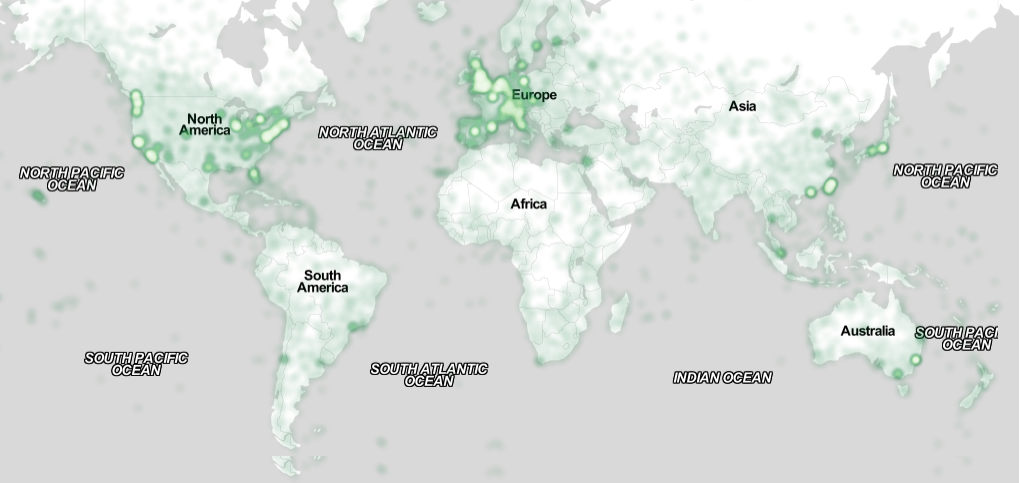
\includegraphics[width=1.75\columnwidth]{figures/map}
%   \caption{In this image, the map maximizes use of space. You can make
%     figures as wide as you need, up to a maximum of the full width of
%     both columns. Note that \LaTeX\ tends to render large figures on a
%     dedicated page. Image: \ccbynd~ayman on
%     Flickr.}~\label{fig:figure2}
% \end{figure*}
% \begin{table}
%   \centering
%   \begin{tabular}{l r r r}
%     % \toprule
%     & & \multicolumn{2}{c}{\small{\textbf{Test Conditions}}} \\
%     \cmidrule(r){3-4}
%     {\small\textit{Name}}
%     & {\small \textit{First}}
%       & {\small \textit{Second}}
%     & {\small \textit{Final}} \\
%     \midrule
%     Marsden & 223.0 & 44 & 432,321 \\
%     Nass & 22.2 & 16 & 234,333 \\
%     Borriello & 22.9 & 11 & 93,123 \\
%     Karat & 34.9 & 2200 & 103,322 \\
%     % \bottomrule
%   \end{tabular}
%   \caption{Table captions should be placed below the table. We
%     recommend table lines be 1 point, 25\% black. Minimize use of
%     table grid lines.}~\label{tab:table1}
% \end{table}
% \begin{figure}
% \centering
%   
\includegraphics[width=0.9\columnwidth]{figures/sigchi-logo}
%   \caption{Insert a caption below each figure. Do not alter the
%     Caption style.  One-line captions should be centered; multi-line
%     should be justified. }~\label{fig:figure1}
% \end{figure}

\balance{}
\bibliographystyle{SIGCHI-Reference-Format}
\bibliography{sample}
\end{document}